
\chapter[Spectral Approximation for Conforming Finite...]{Spectral
  Approximation for Conforming Finite Element 
  Method}\label{chap8} 

\section{The Eigen Value Problem} \label{chap8:sec1}
Let\pageoriginale $V$ and $H$ be Hilbert spaces such that
$V\hookrightarrow H$. We also assume that this imbedding is
compact. Let $\parallel\cdotp\parallel_1$ denote the norm in $V$. The
norm in $H$ is denoted by $\parallel\cdotp\parallel$ or $\parallel
\cdotp\parallel_0$ and the scalar product in $H$ is
$(\cdotp,\cdotp)$. We identify $H$ with its dual $H'$.

Let $a(\cdotp,\cdotp):V\times V\to \mathbb{R}$ be a continuous,
symmetric bilinear form which is $V$-coercive with $\alpha$ as the
coercive constant.

We shall consider the eigen value problem:

Find $u\varepsilon V,\mu\varepsilon \mathbb{R}$ such that 
\begin{equation}\label{chap8:eq8.1}
a(u,v)=\mu(u,v)\; \; \forall \;v \;\varepsilon \;V
\end{equation}

In the following, for an operator $\top: H\to H$, we write 
$$
\parallel\top\parallel=\underset{f\varepsilon H,f\neq 0}{\Sup}
\frac{\parallel\top f\parallel}{\parallel f\parallel}.
$$

\section{The Operator $\top$} \label{chap8:sec2} 
The
operator $\top :H\to V$ is defined as follows. If $f\varepsilon H$
then $\top f$ is defined to be the unique solution of the variational
equation 
$$
a(\top f,v)=(f,v)\; \; \forall \;v \;\varepsilon \;V.
$$

By Lax-Milgram Lemma $\top f$ is well defined for all $f\varepsilon
H$. As the imbedding $V\hookrightarrow H$ is compact we obtain that
$\top$, considered as\pageoriginale an operator from $H$ into $H$, is
compact. The symmetry of $a(\cdotp,\cdotp)$ implies that $\top$ is
symmetric. It is easy to see that \eqref{chap8:eq8.1} is equivalent
to:

Find $u\varepsilon V$ and $\lambda \varepsilon \mathbb{R}$ such that
\begin{equation}\label{chap8:eq8.2}
\top u=\lambda u
\end{equation}

The $\mu$ and $\lambda$ in \eqref{chap8:eq8.1} and \eqref{chap8:eq8.2}
have the relation 
$$
\lambda\mu=1.
$$

From the Spectral Theorem for compact self-adjoint operators we have:

$\Sp(\top)$ is a countable set with no accumulation point other than
zero. Every point in $\Sp(\top)$ other than zero is an eigenvalue of
$\top$ with finite multiplicity. 

\section{Example}\label{chap8:sec3} 
The model problem for \eqref{chap8:eq8.1} is 
$$
V=H_\circ^1(\Omega), \;H=L^2(\Omega)
$$
where $\Omega$ is a smooth bounded open subset of $\mathbb{R}^n$,
$$
a(u,v)=\int\limits_\Omega \nabla u.\nabla v
$$
The compactness of the imbedding $H^1(\Omega)\hookrightarrow
L^2(\Omega)$ is well known. Problem \eqref{chap8:eq8.1} corresponds
to:

Find $u\varepsilon H_\circ^1(\Omega), \mu\varepsilon\mathbb{R}$ such
that 
\begin{equation}\label{chap8:eq8.3}
\begin{cases}
-\Delta u=u\quad\text{in}\quad\Omega,\\
u=0\quad\text{on}\quad\partial\Omega
\end{cases}
\end{equation}\pageoriginale
We note that $\top$ is the inverse of $-\Delta$.

\section{Approximate Problem}\label{chap8:sec4} Let
$V_h\hookrightarrow V$ be a finite element subspace of $V$. We
consider the approximate eigen value problem:

Find $u_h\;\varepsilon \;V_h,\;\mu_h\;\varepsilon \;\mathbb{R}$ such
that 
\begin{equation}\label{chap8:eq8.4}
a(u_h,v_h)=\mu_h(u_h,v_h)\; \; \forall \;v_h\;\varepsilon \;V_h 
\end{equation}

Here again, we introduce an operator $\top_h:H\to H$ where $\top_hf$
is the unique solution of 
\begin{equation}\label{chap8:eq8.5}
a(\top_hf,v_h)=(f,v_h)\; \; \forall \;v_h\;\varepsilon \;V_h.
\end{equation}

As in the continuous case, we have $\parallel\top_h\parallel\leq
c/\alpha$ which shows that $\top_h$ is uniformly bounded. Again
\eqref{chap8:eq8.4} is equivalent to:

Find $u_h\varepsilon V_h$ and $\lambda_h=1/\mu_h$ such that 
\begin{equation}\label{chap8:eq8.6}
\top_h\;u_h=\lambda_h\;u_h
\end{equation}

It is obvious that $\top_h$ is a self-adjoint, compact operator. 

We assume that 
\begin{equation}\label{chap8:eq8.7}
\parallel\top-\top_h\parallel\leq\varepsilon(h)
\end{equation}
and 
\begin{equation}\label{chap8:eq8.8}
\parallel (\top-\top_h)\;f\parallel \leq e(h)
\end{equation}
for\pageoriginale all smooth $f$ and $\top f$. Further, we assume 
\begin{equation}\label{chap8:eq8.9}
0\leq e(h)\leq\;\varepsilon (h)\quad\text{and}\quad\varepsilon(h)\to 0
\end{equation}
\begin{Example*}
Let 
$$
V_h=\{v_h\;\varepsilon \;H_\circ^1(\Omega):v_h|_K\;\varepsilon
\;\mathbb{P}_k(K), \;K\;\varepsilon \;T_h\}
$$
where $T_h$ is a regular family of triangulations of $\Omega$. We have
(\cf Chapter \ref{chap5})
\begin{equation}\label{chap8:eq8.10}
\parallel\top f-\top_hf\parallel_{0,\Omega}\leq\ch^{s+1}\parallel f
\parallel_{s-1,\Omega}, 1\leq s\leq k,
\end{equation}
provided that $\Omega$ is a convex polygon and that 
\begin{equation}\label{chap8:eq8.11}
\parallel\top f\parallel_{s+1}\leq c\parallel f\parallel_{s-1,\Omega}.
\end{equation}

From GRISVARD \cite{key22} this is atleast true for $s=1$, which shows 
that $\varepsilon(h)=\ch^2$ and $e(h)=0(h^{k+1})$.
\end{Example*}

\section{Convergence and Error Estimate for the Eigen
  Space.} \label{chap8:sec5} Assumption \eqref{chap8:eq8.7}
\eqref{chap8:eq8.9} show that $\top_h\to\top$ in norm.

From KATO \cite{key26} (Chapter \ref{chap5}. Section \ref{chap4:ssec4.3}) we
know that the spectrum of $\top_h$ converges to the spectrum of $\top$
in the following sense: For all non-zero $\lambda\varepsilon
\Sp(\top)$ with multiplicity $m$ and for each $h$ such that
$\varepsilon(h)<d/2$, where 
$$
d=\min\limits_{\lambda'\varepsilon\Sp(\top)}|\lambda-\lambda'|,
$$
there exist exactly $m$ eigen values $\lambda_{ih}\varepsilon
\Sp(\top_h)$ (counted according to multiplicity) such that 
\begin{equation*}
|\lambda-\lambda_{ih}|\leq\;\varepsilon(h).
\end{equation*}\pageoriginale

Let $\Gamma=\{z\varepsilon C:|z-\lambda|=d/2\}$. We know that 
\begin{align}
&P=-\frac{1}{2\pi i}\int\limits_\Gamma
R_z(\top)\,dz,\label{chap8:eq8.12}\\
&P_h=-\frac{1}{2\pi i}\int\limits_\Gamma R_z(\top_h)\,dz,\;\varepsilon
(h)<d/2, \label{chap8:eq8.13}
\end{align}
where $R_z(\top)=(\top-z)^{-1}$, are the spectral projections on to
the eigen-spaces $E$ and $E_h$ associated with $\lambda$ and
$\lambda_{ih}$'s. The dimension of each of the spaces $E$ and $E_h$ is
$m$ (See KATO \cite{key26}, Chapter \ref{chap4}, Section
\ref{chap4:ssec4.3}). 
\setcounter{lem}{0}
\begin{lem}\label{chap8:lem1}
For $u\varepsilon E$, we have 
\begin{equation}\label{chap8:eq8.14}
\parallel u-P_hu\parallel \leq c_2\parallel
\;(\top-\top_h)\;u\parallel.
\end{equation}
\end{lem}

\begin{proof}
We consider 
\begin{align*}
R_z(\top)-R_z(\top_h) &= R_z(\top_h)(\top_h-z)R_z(\top)-R_z(\top_h)
(\top-z)R_z(\top)\\ 
&= R_z(\top_h)(\top_h-\top)R_z(\top).
\end{align*}
Hence
$$
P-P_h=-\frac{1}{2\pi i}\int\limits_\Gamma R_z(\top_h)(\top_h-\top)R_z
(\top)\,dz.
$$
Let $u\varepsilon E$. Then we have 
$$
Pu=u,\top u=\lambda u\quad\text{and}\quad
R_z(\top)u\frac{1}{\lambda-z}u. 
$$
Therefore\pageoriginale
$$
u-P_hu=-\frac{1}{2\pi i}\int\limits_\Gamma \frac{R_z(\top_h)}
{\lambda-z}\,dz\;(\top-\top_h)\;u.
$$

We show that the integral on the right is bounded. Indeed, for
$z\varepsilon\Gamma$ and $\varepsilon(h)<d/2$ we have 
\begin{align*}
\top_h-z &= \top_h-\top+\top-z\\
&= ((\top_h-\top)\;R_z(\top)+I)\;(\top-z),
\end{align*}
which implies
$$
R_z(\top_h)=R_z(\top)\;(I+A_h)^{-1},
$$
where 
$$
A_h=(\top_h-\top)\;R_z(\top).
$$

If $P(\top)$ denotes the resolvent set of $\top$ then, as $R_z(\top)$
is continuous in $z\varepsilon P(\top)$ and $\Gamma$ is a compact
subset of $P(\top)$, we obtain 
$$
\parallel R_z(\top)\parallel \leq c_1\quad\text{for all }
z\;\varepsilon \Gamma,
$$
and $\parallel A_h\parallel\leq c_1\varepsilon(h)$, where $c_1$ is a
constant. This implies
$$
\parallel(I+A_h)^{-1}\parallel\leq 2\quad\text{for}\quad\varepsilon(h)
\leq\frac{1}{2c_1}.
$$
Thus
$$
\parallel u-P_hu\parallel\leq c_2\parallel
\;(\top-\top_h)\;u\parallel.
$$
\end{proof}

\begin{lem}\label{chap8:lem2}
If the eigen vectors in $E$ are smooth enough, we have 
\begin{equation}\label{chap8:eq8.15}
\delta(E,\;E_h)\leq c\;e(h),
\end{equation}\pageoriginale
where
$$
\delta(E,\;E_h)=\Sup\;\{d(u,E_h):\;u\;\varepsilon \;E,\parallel
u\parallel=1\}.
$$
\end{lem}

\begin{Remark}\label{chap8:Rem1}
In this chapter we follow closely OSBORN \cite{key34}. We will use the result:
``In a Hilbert space $H, \delta(E, E_h)=\delta(E_h, E)$''. Osborn,
however, considers the more general case of a non-self-adjoint
operator in a Banach space, which involves more complicated arguments.
\end{Remark}

\section{Error Estimates for the Eigen Values.} \label{chap8:sec6}
Let $Q_h=P_h|_E$, the restriction of $P_h$ to $E$. Then $Q_h$ maps $E$
into $E_h$. We prove that $Q_h$ is invertible for small $h$.

Indeed, for $h$ small enough we have $\dim E= \dim E_h$.

Let $f\varepsilon E$ be such that $Q_hf=0$. Then
$$
\parallel f\parallel =\parallel f-Q_hf\parallel =\parallel f-P_hf \parallel
\leq c_2\varepsilon(h)\parallel f\parallel,
$$
where we have used Lemma \ref{chap8:lem1}. Therefore, for $c_2
\varepsilon(h)<1$ we have $\parallel f\parallel=0$. Hence $Q_h$ is
invertible for $\varepsilon(h)<\min(d/2, 1/c_2)$. 

Let us evaluate $\parallel Q_h^{-1}\parallel$. If $f\varepsilon E$ with
$\parallel f\parallel =1$, then
$$
1-\parallel Q_hf\parallel \leq \parallel f-P_hf\parallel \leq c_2
\;\varepsilon(h).
$$
Therefore
$$
\parallel Q_hf\parallel \geq 1/2,\quad\text{if}\quad\varepsilon(h)
\leq 1/2c_2
$$\pageoriginale
and
$$
\parallel Q_h^{-1}\parallel \leq 2,\quad\text{for}\quad\varepsilon
(h)\leq 1/2c_2.
$$

Let $\hat{\top}_h:E\to E$ be defined by
$$
\hat{\top}_h=Q_h^{-1}\top_h\;Q_h.
$$
The eigenvalues of $\hat{\top}_h$ are again $\lambda_{ih}, i=1,
2,\ldots,m$ (but the eigenvectors of $\hat{\top}_h$ are different from
those of $\top_h$).

Let $W_{jh}\varepsilon E, \parallel W_{jh}\parallel =1$ be an eigen
vector of $\hat{\top}_h$ associated with the eigen value
$\lambda_{jh}$. Therefore,
\begin{align*}
\lambda-\lambda_{jh} &= ((\lambda-\lambda_{jh})\;w_{jh},\;w_{jh})\\
&= ((\top-\top_h)\;w_{jh},\;w_{jh})\\
&\leq \underset{\phi\varepsilon E,\parallel\phi\parallel=1}{\Sup}
\{((\top -\top_h)\;\phi,\phi)\}.
\end{align*}
Now 
\begin{align*}
\top -\hat{\top}_h &=\top-Q_h^{-1}\top_h\;Q_h=\top-Q_h^{-1}\;\top_h\;
P_h\\ 
&= \top-Q_h^{-1} \;P_h \;\top_h.
\end{align*}
Hence
\begin{equation}\label{chap8:eq8.16}
\top-\hat{\top}_h=Q_h^{-1}\;P_h\;(\top-\top_h),
\end{equation}
since $P_h$ commutes with $\top_h$ and $Q_h^{-1}P_hu=u$ for
$u\varepsilon E$. Hence 
$$
\parallel (\top-\hat{\top}_h)\phi\parallel\leq 2\parallel
(\top-\top_h)\phi \parallel\quad\text{for all }\phi \varepsilon E
$$
since 
$$
\parallel Q_h^{-1}\parallel \leq 2,\parallel P_h\parallel \leq 1\quad
\text{for}\quad\varepsilon(h)\leq 1/2c_1.
$$\pageoriginale
Therefore
\begin{equation}\label{chap8:eq8.17}
|\lambda-\lambda_{jh}|\leq 2e(h)\quad\text{for}\quad\varepsilon(h)
\leq\min(1/2c_1, \,d/2)
\end{equation}

\noindent{\bf Application.} In the example given in Section \ref{chap8:sec3},
where $\top$ is the inverse of the negative Laplace operator, we get 
\begin{align}
|\lambda-\lambda_{ih}| &\leq \ch^{k+1}, \;1\leq i\leq
m, \label{chap8:eq8.18}\\
d(E, E_h) &\leq \ch^{k+1}, \label{chap8:eq8.19}
\end{align}
since $e(h)\leq\ch^{k+1}$ provided that the eigen functions in $E$ are
in $H^{k+1}$ (This may happen even though $\Omega$ is a polygon: If
$\Omega =]0,1[^2$ the eigen functions are known explicitly and they
are $C^\infty$. In fact, the eigen functions are 
$$
u_{nm}=\Sin \;n\pi x.\Sin \;m\pi x.
$$

However, the error estimate for $|\lambda-\lambda_{jh}|$ can be
improved as will be shown in the following section. One indeed has 
$$
|\lambda-\lambda_{jh}|\leq\ch^{2k}.
$$

\section[Improvement of the Error Estimate for the...]{Improvement of
  the Error Estimate for the\hfil\break Eigen 
  Values.} \label{chap8:sec7} We denote by $S_h$ the projection on
$E_h$ along $E^\bot$. We notice that 
$$
R_h=Q_h^{-1}P_h
$$
is the projection on $E$ along $E_h^\bot$. 
\begin{figure}[H]
\centering
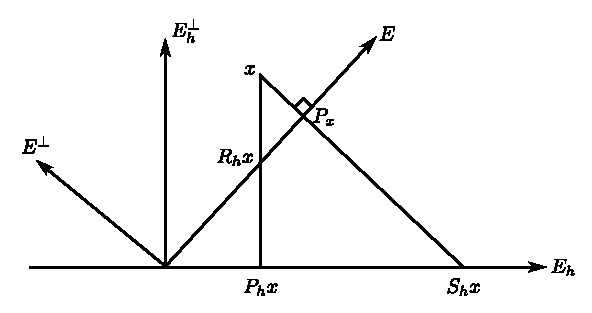
\includegraphics{figure/fig8.1.eps}
\caption{}\label{fig8.1}
\end{figure}\pageoriginale
\noindent
$S_h$ and $R_h$ are related by 
\begin{lem}\label{chap8:lem3}
$S_h=R_h^*$.
\end{lem}

\begin{proof}
For $u, v \varepsilon H$, we have 
\begin{align*}
(u,S_h\phi) &= (P_hu,S_h\phi),\quad\text{since}\quad P_hS_h=S_h\quad
\text{and}\quad P_h^*=P_h,\\
&= (P_hR_hu,S_h\phi),\text{ since}\quad R_h \text{ is the
projection on $E$ along } E_h^\bot;\\
&= (R_hu, S_h\phi)\\
&= (R_hu,PS_h\phi),\quad\text{since}\quad PR_h=R_h\quad\text{and}
\quad P=P^*,\\
&= (R_hu, P\phi),\quad\text{since}\quad PS_h=P,\\
&= (R_hu,\phi).
\end{align*}
\end{proof}

We will now prove a Lemma which will give an upper bound for
$\parallel P-S_h\parallel$.

\begin{lem}\label{chap8:lem4}
We have 
\begin{equation}\label{chap8:eq8.20}
\parallel P-S_h\parallel \leq \frac{\delta(E_h,E)}{1-\delta (E_h,E)} 
\end{equation}\pageoriginale
\end{lem}

\begin{proof}
Since $S_h$ is the projection on $E_h$ along $E^\bot$ we have
$P=PS_h$. If $x\varepsilon E_h$ and $\parallel x\parallel =1$ then 
$$
\parallel x-Px\parallel=d(x,E)\leq \underset{x\varepsilon E_h,
\parallel x\parallel=1}{\Sup}d(x,E)=\delta(E_h,E).
$$
Therefore,
\begin{equation}\label{chap8:eq8.21}
\parallel y-Py\parallel\leq\delta(E_h,E)\parallel y\parallel\quad
\text{for all } y\;\varepsilon E_h
\end{equation}
Now, for any $x\varepsilon H$,
\begin{align*}
\parallel S_hx\parallel &\leq \parallel S_hx-PS_hx\parallel +\parallel
PS_hx\parallel\\
&\leq \delta(E_h,E)\parallel S_hx\parallel + \parallel Px\parallel.
\end{align*}
Thus
\begin{equation}\label{chap8:eq8.22}
\parallel S_hx\parallel \leq \frac{1}{1-\delta(E_h,E)}\parallel
x\parallel 
\end{equation}
Hence we obtain
\begin{align*}
\parallel(P-S_h)x\parallel &= \parallel PS_hx-S_hx\parallel\\
&\leq\delta(E_h,E)\parallel S_hx\parallel,\quad\text{by
\eqref{chap8:eq8.21}},\\
&\leq\frac{\delta(E_h,E)}{1-\delta(E_h,E)}\parallel x\parallel,
\quad\text{using \eqref{chap8:eq8.22}}
\end{align*}
Therefore 
$$
\parallel P-S_h\parallel \leq \frac{\delta(E_h,E)}{1-\delta(E_h, E)}. 
$$
\end{proof}

Finally we have from \eqref{chap8:eq8.16}, 
\begin{align*}
((\top-\hat{\top}_h)\;\phi,\phi) &= (R_h\;(\top-\top_h)\phi,\phi)\\
&= ((\top-\top_h)\;\phi,\;S_h\phi)\\
&= ((\top-\top_h)\phi,\phi)+((\top-\top_h)\phi,S_h\phi-\phi),
\end{align*}\pageoriginale
where $\phi\varepsilon E$ and $\parallel\phi\parallel=1$.

\noindent For $\phi\varepsilon E$, using Lemma \ref{chap8:lem4} and
Lemma \ref{chap8:lem2}, we obtain
$$
\parallel\phi-S_h\parallel \leq \frac{\delta(E_h,E)}{1-\delta(E_h, E)}
\leq k\;e(h),
$$
for sufficiently small $h$, where $k$ is a constant.

We know that for all $\phi\varepsilon E$ with $\parallel\phi\parallel
=1$
$$
\lambda-\lambda_{ih}=((\top-\hat{\top}_h)\;\phi,\phi).
$$
Hence 
$$
|\lambda-\lambda_{ih}|\leq\underset{\phi\varepsilon E,\parallel\phi
\parallel =1}{\Sup}((\top-\top_h)\phi,\phi)+k(e(h))^2.
$$
Thus we have proved 
\setcounter{THM}{4}
\begin{THM}\label{chap8:THM5}
When $E$ is a smooth subset of $H$ and $h$ is sufficiently small we
have 
\begin{equation}\label{chap8:eq8.23}
|\lambda-\lambda_{ih}|\leq\underset{\phi\varepsilon E,\parallel\phi
\parallel=1}{\Sup}((\top-\top_h)\phi,\phi)+k(e(h))^2,
\end{equation}
where $k$ is a constant.
\end{THM}

\medskip
\noindent{\textbf{Application.}}
 In\pageoriginale the case of the
example in Section \ref{chap8:sec3}, we give an estimate of 
$$
\alpha_h=\underset{\phi\varepsilon E,\parallel\phi\parallel=1} {\Sup}
((\top-\top_h)\phi,\phi).
$$

Let $w$ be the solution of 
\begin{equation}\label{chap8:eq8.24}
a(v,w)=(\phi,v)\; \; \forall \;v \;\varepsilon \;V,
\end{equation}
where $\phi\varepsilon E$ and $\parallel\phi\parallel=1$.

\noindent We have 
\begin{align*}
((\top-\top_h)\phi,\phi) &= a((\top-\top_h)\phi,\;w)\\
&= a((\top-\top_h)\phi,w-v_h)\quad\text{for all } v_h
\;\varepsilon \;V_h,
\end{align*}
since
$$
a((\top-\top_h)\phi,\;v_h)=0\quad\text{for all } v_h \;\varepsilon
\;V_h.
$$

If $w\varepsilon H^{k+1}(\Omega)$, we get
$$
\parallel w-v_h\parallel_1\leq\ch^k\parallel w\parallel_{k+1} \leq
\ch^k\parallel\phi\parallel_{k-1},
$$
using regularity theorem and the error estimates in Chapter
\ref{chap5}.

Since $E$ is finite-dimensional there exists a constant $c$ such that 
$$
\parallel\phi\parallel_{k-1}\leq c\parallel\phi\parallel =c.
$$

Finally, we have 
\begin{gather*}
\alpha_h\leq\ch^k\;\parallel(\top-\top_h)\phi\parallel_1\\
\leq\ch^{2k},
\end{gather*}
provided\pageoriginale that $E\subset H^{k+1}$.

Thus we have proved

\begin{THM}\label{chap8:THM6}
For the model problem (See Section \ref{chap8:sec3}) we have 
$$
|\lambda-\lambda_{ih}|\leq\ch^{2k},
$$
provided $E\subset H^{k+1}(\Omega)$, the solution of
\eqref{chap8:eq8.24} is in $H^{k+1}(\Omega)$ and $h$ is small.
\end{THM}

\setcounter{REM}{1}
\begin{REM}\label{chap8:rem2}
Error estimates for the semi-discrete approximation to parabolic
equation of the form
\begin{gather*}
\left(\frac{du}{dt},v\right)+a(u,v)=(f,v)\quad\text{for all } v
\;\varepsilon \;V,\\
u(0)=v_\circ,\;v_\circ \;\varepsilon \;V,
\end{gather*}
can be obtained using spectral approximation. The reader is referred
to THOMEE \cite{key44}, \cite{key45}.
\end{REM}
